Se sabe que el modelo estándar proporciona una descripción incompleta de la física de partículas y una serie de extensiones del \ME ~ predicen la existencia de nuevos bosones de luz. Un posible modelo de búsqueda independiente para la producción en pareja de un bosón ligero que se descompone en un par de muones. 

Un ejemplo simple de producción de pares en colisiones protón-protón (pp) es $pp \rightarrow h \rightarrow 2a + \chi \rightarrow 4\mu + \chi$, donde $h$ es un bosón de Higgs, a es el nuevo bosón neutro ligero, y X son partículas de espectador que se predicen en varios modelos. Si bien la producción a través del bosón h es posible, no se requiere en la búsqueda presentada aquí: el único requisito es que un par de bosones de luz idénticos sean vértices comunes de datos y un bosón de luz de decaimiento se descomponga posteriormente en un par de muones. Estos pares de muones se denominan ``dimuones'', el vértigo y los nuevos vértices de producción de bosones ligeros pueden ser desplazados. La naturaleza genérica de esta firma significa que cualquier límite establecido en el producto de la sección transversal, la fracción de ramificación a los dimuons al cuadrado, y la aceptación es independiente del modelo; Por lo tanto, puede ser reinterpretado en el contexto de modelos específicos.


\subsection{Definición}

Entre sus observaciones más recientes \cite{ams:cern} se ha reportado un flujo de positrones anómalo que tiene una posible explicación en el proceso de aniquilación de partículas de materia oscura, donde se libera energía en forma de positrones. Dicho flujo anómalo puede observarse
a partir de los 25 GeV en la Figura \ref{fig:AMS_positronflux} donde también se presenta una comparación con otros experimentos que observan similar comportamiento.

\begin{figure}[ht!]
    \centering
    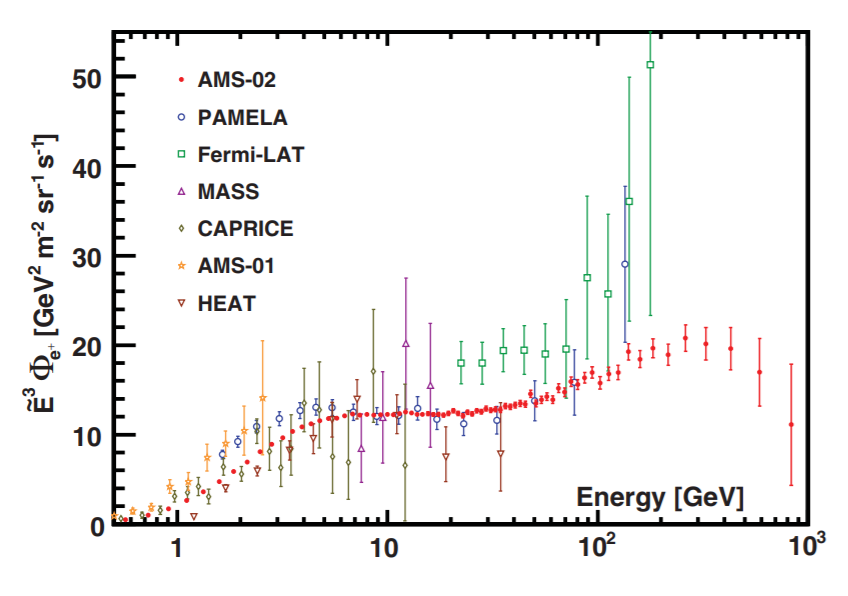
\includegraphics[width=0.75\textwidth]{Fisica_de_Particulas/imagenes/AMS_positronflux.png}
    \caption{Flujo de positrones medido por el experimento AMS-02, comparado con los experimentos PAMELA, Fermi-LAT, MASS, CAPIRCE, AMS-01 y HEAT.}
    \label{fig:AMS_positronflux}
\end{figure}

Estas observaciones cosmológicas han motivado a los físicos teóricos de altas energías a postular nuevos modelos en los cuales la composición de la materia oscura se pueda entender por medio de nuevas partículas elementales no descritas en el modelo estándar y que sin embargo podrían estar siendo producidas en los aceleradores de partículas modernos como el Gran Colisionador de Hadrones en Ginebra, Suiza. Los modelos propuestos se encuentran en la categoría que se conoce como extensiones al modelo estándar y por lo general involucran la existencia de nuevas partículas cuyas fuerzas e interacciones están descritas por alguna variación de la teoría cuántica de campo, lo que sugiere que sus mecanismos de producción y propiedades pueden ser estudiados por el formalismo de la física de partículas y la parte experimental por medio de los detectores de partículas con métodos de recolección de datos, selección de eventos y técnicas estadísticas para el análisis y extracción de posibles señales.

\subsection{Formulación Teórica}



En el SUSY oscuro, $U(1)$ (una simetría global de Peccei–Quinn) se rompe, dando lugar a fotones oscuros ($g_\gamma$) que se acoplan débilmente a las partículas SM a través de una pequeña mezcla cinética entre los fotones. El neutralino más ligero $n_1$ en el espectro visible (opuesto al escondido) de SUSY ya no es estable y puede descomponerse a través de procesos como $n_1\longrightarrow  n_D + \gamma_D$, donde $n_D$ es un fermión oscuro (neutralino oscuro) que escapa a la detección. En estos modelos, las desintegraciones de $\gamma_D$ a menudo están mediadas por interacciones muy débiles con el SM, y en gran parte del espacio de parámetros disponible tienen una larga vida útil. Si la SUSY oscura se realiza en la naturaleza, la descomposición de los fotones oscuros podría ocurrir a cierta distancia dentro del detector, o incluso potencialmente fuera de este.

La falta de un exceso de antiprotones en las mediciones del espectro de rayos cósmicos limita la masa de $\gamma$ a $\leq 2m_p$. Suponiendo que $\gamma_D$ solo puede descomponerse en partículas SM, la fracción de ramificación $(\gamma_D\rightarrow \mu^+\mu^-)$ puede ser tan grande como 45\% esto dependiendo de $m_{\gamma_D}$. Si el acoplamiento a las partículas SM está altamente suprimido, entonces la masa $m_{\gamma_D}$ también puede tener una vida útil no despreciable y recorrer cierta distancia antes de la descomposición. Por lo tanto, es importante acomodar la posibilidad de fotones oscuros de larga duración en nuestras búsquedas.

Las nuevas fuerzas ocultas en los escenarios de Dark SUSY pueden acoplarse a la hipercarga SM a través de un término de mezcla cinética en lagrangiano:
\begin{equation}
\label{an-15-455:ec3}
L_{KM}\backsim \dfrac{\epsilon}{2} F_{\mu v}^{\gamma} F^{\mu v}
\end{equation}
donde $F_{\mu v}^{\gamma} = \partial_\mu A_v^{D} -\partial_v A_\mu^D$ y $A^D$ es el campo de calibre oscuro [37-39]. Si el $A_D$ es masivo, entonces las partículas SM adquieren una carga adicional $\epsilon e$ bajo la interacción oscura. Tenga en cuenta que en los escenarios típicos del SUSY oscuro con mezcla cinética del parámetro $\epsilon$ está dentro del rango $10^{-8}-10^{-2}$. 

Se prueba que debido a la mezcla cinética, el fotón oscuro se descompondrá en leptones SM con un ancho parcial dado por:
\begin{equation}
\label{an-15-455:ec4}
\Gamma_{\gamma_D \rightarrow \vec{l}l} = \dfrac{1}{3}\alpha \epsilon^2 m_{\gamma_D} \sqrt{1- \dfrac{4m_l^2}{m_{\gamma_D}^2}}
\left( 1 + \dfrac{2m_l^2}{m_{\gamma_D}^2}\right) 
\end{equation}
donde $m_l$ es la masa del leptón y los diferentes modos de descomposición comienzan desde $m_{\gamma_D} > 2 m_l$. Además, el fotón oscuro se descompondrá en hadrones SM para masas $m_{\gamma_D} > 2 m_\pi$, con ancho parcial dado por:
\begin{equation}
\label{an-15-455:ec5}
\Gamma_{\gamma_D} \rightarrow = \dfrac{1}{3} \alpha \epsilon^2 m_{\gamma_D} \sqrt{1 -\dfrac{4 m_{\mu^2}}{m_{\gamma_D}^2}} \left( 1 + \dfrac{2 m_\mu^2}{m_{\gamma_D}^2}\right) R(s = m_{\gamma_D}^2)
\end{equation}

donde $R = \sigma_{e^+ e^- \rightarrow hadrons} / \sigma_{e^+ e^- \rightarrow \mu^+ \mu^-}$. Los datos de la sección transversal hadrónica están disponibles en la bibliografia científica resultado de varias mediciones experimentales, resultado de estas pero solo se mide a partir de $\sqrt{s}= 0.36G ~ eV / c^2$, que está por encima del umbral $2 m_\pi = 0.28~GeV / c^2$. Por lo tanto, en la región donde $ < ~ 0.36~GeV / c^2$, usamos la sección transversal para $e^+e^- \rightarrow \pi^+\pi^-$. Finalmente, para la región donde $\sqrt{s} < 2 m_\pi$, sumamos solo los anchos parciales de leptones.

\begin{table}[h!]
  \begin{center}
   \caption{Ancho total y $f(m_{\gamma_D})$.}
    \label{an-15-455:tb1}
    \begin{tabular}{|l|c|c|c|c|c|c|c|c|r|} % <-- Alignments: 1st column left, 2nd middle and 3rd right, with vertical lines in between
		\hline 		
		&\multicolumn{9}{c|}{$m_{\gamma_D}, ~GeV/c^2$}\\		
		\hline 
		&0.25 & 0.275 & 0.3 & 0.4 & 0.7 & 1 & 1.5 & 2 & 8.5\\
		\hline       
       	$\Gamma_{\gamma_D Total/\epsilon^2}[MeV]$ & 1 & 1.2 & 1.9 & 2.1 & 11.4 & 8.0 & 15.5 & 20.3 & 114.6 \\
       	\hline 
       	$f(m_{\gamma_D})~[GeV^{-1}]$ & 952.9 & 817.2 & 538.9 & 480.2 & 87.4 & 125.1 & 64.6 & 49.2 & 8.7 \\
      	\hline      
    \end{tabular}
  \end{center}
\end{table}

Según las expresiones (\ref{an-15-455:ec4}) y (\ref{an-15-455:ec5}), las dependencias del ancho parcial de $\epsilon$ y $m_{\gamma_D}$ pueden factorizarse como $ (\Gamma_{\gamma_D}/\epsilon^2)^{-1}= f (m_{\gamma_D})$, donde $f (m_{\gamma_D})$ es solo dependiente de la masa del fotón oscuro. Los anchos parciales para los diferentes modos de decaimiento del fotón oscuro y su ancho total (todos divididos por $\epsilon^2$ para demostrar solo la dependencia de los anchos con $m_{\gamma_D}$) se muestran en la Tab. \ref{an-15-455:tb1} %y Fig. \ref{an-15-455:fig4}
. La relación de ramificación para la descomposición del fotón oscuro a un par de muones $B_{\gamma_D\rightarrow \mu\mu} = \Gamma_{\gamma_D\rightarrow \mu\mu} /\Gamma_{\gamma_D Total}$ no depende de $\epsilon$, y se muestra %en la Fig. \ref{an-15-455:fig4} 
como función de $m_{\gamma_D}$. Esta relación de ramificación $B_{\gamma_D\rightarrow\mu\mu}$ tiene un mínimo en $m_{\gamma_D}\thicksim 0.8 ~ GeV/ c^2$, donde predomina el decaimiento del fotón oscuro en hadrones. 
%Figura 4: Izquierda: Ancho total considerando los diferentes modos de desintegración del fotón oscuro, normalizado por e2. Derecha: ¡Relación de ramificación para gD! mm modo de decaimiento. Las expresiones para los anchos parciales permiten el cálculo de la vida útil del fotón oscuro a través de:

\begin{figure}
    \centering
    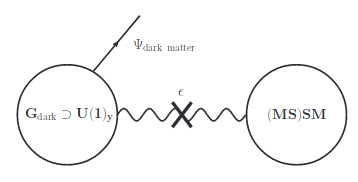
\includegraphics[width=0.4\textwidth]{Fisica_de_Particulas/imagenes/sketch_darksector.png}
    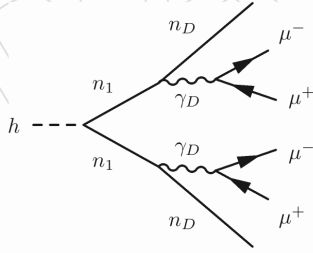
\includegraphics[width=0.4\textwidth]{Fisica_de_Particulas/imagenes/darksusy_feynman.png}
    \caption{ Ilustración esquemática de la conexión entre el sector oscuro y el modelo estándar, los cuales están conectados mediante un término de mezcla dinámica.}
    \label{fig:sketch_darksector}
\end{figure}



Las expresiones para los anchos parciales permiten el cálculo del tiempo de vida del fotón oscuro:
\begin{eqnarray}
\label{an-15-455:ec6}
\tau_{\gamma_D} = \dfrac{}{\Gamma_{\gamma_D Total}} =\dfrac{1}{\Gamma_{\gamma_D \rightarrow e^+ e^-} + \Gamma_{\gamma_D \rightarrow \mu^+ \mu^-} + \Gamma_{\gamma_D \rightarrow hadrons }}
\end{eqnarray}
El tiempo de vida está directamente relacionada con el parámetro $\epsilon$ y la masa del fotón oscuro se obtiene:
\begin{eqnarray}
\label{an-15-455:ec7}
\tau_{\gamma_D}(\epsilon,m_{\gamma_D}) =\dfrac{1}{\epsilon^2}\times f(m_{\gamma_D})
\end{eqnarray}
Es conveniente representar el tiempo de vida $\tau_{\gamma_D}$ en unidades de distancia $c\tau_{\gamma_D}$, donde $c$ es la velocidad de la luz. También es conveniente medir $c\tau_{\gamma_D}$ en milímetros porque la sensibilidad del análisis a esta variable es $\sigma(mm)$. Las restricciones sobre $\epsilon$ y la masa del fotón oscuro podrían obtenerse a partir de las restricciones sobre la vida útil del fotón oscuro porque están directamente relacionadas entre sí, como ya se comprobo anteriormente.

El diagrama de Feynman del proceso del SUSY oscuro  $h \rightarrow 2n_1 \rightarrow 2n_D + 2\gamma_D \rightarrow 2n_D + 4\mu$ se muestra en la Fig. \ref{fig:sketch_darksector}. Este modelo de referencia es solo un escenario posible, y se elige como una representación única de un rango muy amplio de espacio de parámetros disponibles. Este modelo simple del sector oscuro se puede ampliar de varias maneras; versiones más complejas involucran otros bosones oscuros de Higgs, $W$ y $Z$. También hay muchos otros procesos permitidos, como por ejemplo $pp \leftarrow h \leftarrow Z_D Z / Z_D Z_D / Z_a \leftarrow 4\mu$. En este análisis representamos los resultados de una manera que permite reinterpretaciones adicionales en el marco de otros modelos.a




